\documentclass{article}


\usepackage{amsmath}
\usepackage{amssymb}
\usepackage{hyperref}
\usepackage{natbib}
\usepackage{xcolor}
\usepackage{graphicx}

\newcommand{\dom}{\ensuremath{\mathbf{dom}}}

\hypersetup{
    colorlinks,
    linkcolor={red!50!black},
    citecolor={blue!50!black},
    urlcolor={blue!80!black}
}

\graphicspath{ {.} }

\begin{document}

\section{Basic Maths}

\subsection{Line Segments}

Given two points, $x_1 \ne x_2$ in $\mathbb{R}^n$ we can define the line that passes through them as (with $\theta \in \mathbb{R}$),

\begin{align}
    y = \theta x_1 + (1 - \theta) x_2 \\
    y = x_2 + \theta ( x_1 - x_2)
\end{align}

\noindent
In either of these formulations, the interpretation is that
$\theta = 0 \rightarrow x_2$,
$\theta = 1 \rightarrow x_1$,
$0 < \theta < 1$ is between the two points,
and other values of $\theta$ are outside.

\subsection{Affine Sets}

A set $C$ is affine if the line through any two points in $C$ lies in $C$. i.e.,

\begin{equation}
    x_2 + \theta (x_1 - x_2 ) \in C \text{ for all } \theta \in \mathbb{R}
\end{equation}

Note that an affine set (is always?) infinite. Consider the simple case of, $x_1 = 0$, $x_2 = 1$. The affine set of these two points is the entire X axis.

We can construct an affine set with more than two points. Given $x_1 \cdots x_k \in C$ and the corresponding $\theta_1 + \cdots + \theta_k = 1$, $C$ is affine if all,

\begin{equation}
    x_1 \theta_1 + \cdots + x_k \theta_k = y \in C
\end{equation}

\subsection{Convex Sets and Hulls}

A set $C$ is convex if every line segment between two points in $C$ is also in $C$.
This is {\em more\/} restrictive than for an affine set (which included all points on the line segment going through, not just between, the points) as it restricts $0 \leq \theta \leq 1$.
Thus, every affine set is also convex.

\begin{figure}[h!]
    \centering
    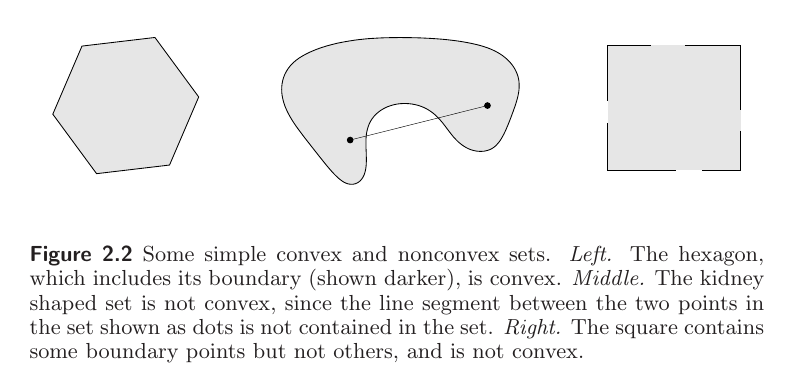
\includegraphics[width=1\textwidth]{./figures/ConvexSetExamples.png}
\end{figure}

As with affine sets, convex sets can be defined by more than two points.
We call a point of the form

\begin{align}
    x_1 \theta_1 + \cdots + x_k \theta_k & = y \\
    \theta_1 + \cdots + \theta_k         & = 1
\end{align}

a {\em convex combination\/} of the points $x_1, \cdots, x_k$.

the smallest convex set that contains those points is called the {\em convex hull\/}.

\begin{figure}[h!]
    \centering
    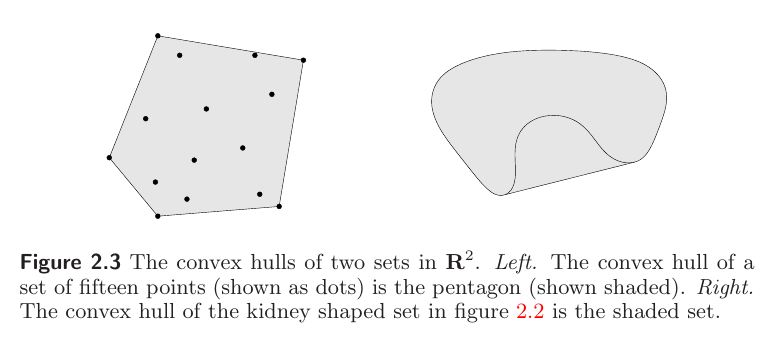
\includegraphics[width=1\textwidth]{./figures/ConvexHullExamples.png}
\end{figure}

This explains why this method is called convex; the resulting set is convex.

\subsection{Cone Sets}

\subsection{Examples}

\begin{itemize}
    \item Any single point, any $\mathbb{R}^n$, and the empty set are all affine
    \item An infinite line is affine (and therefore also convex).
    \item A line segment is convex, but not affine.
\end{itemize}

\subsection{Quadratic Forms}

I'm comfortable with the idea that a quadratic function in one variable looks like, $a x^2$.
In two variables a quadratic function can look like $a x_1^2 + 2 b x_1 x_2 + c x_2^2$ (where we would usually be using $x, y$ as the indexes, but we use $x_1, x_2$ because it will make more sense later).
However, we can rewrite this as,

\begin{equation}
    x^T \begin{bmatrix}
        a & b \\
        b & c \\
    \end{bmatrix} x = x^T  \begin{bmatrix}
        ax_1 + bx_2 \\
        bx_1 + cx_2 \\
    \end{bmatrix}  = ax_1^2 + bx_1x_2 + bx_1x_2 + cx_2^2 = ax_1^2 + 2bx_1x_2 + cx_2^2
\end{equation}

\noindent
This extends to higher dimensions, e.g.

\begin{equation}
    x^T \begin{bmatrix}
        a & b & c \\
        b & d & e \\
        c & e & f \\
    \end{bmatrix} x = a x_1^2 + 2 b x_1 x_2 + 2 c x_1 x_3 + d x_2^2 + 2 e x_2 x_3 + f x_3^2
\end{equation}

\begin{figure}[h!]
    \centering
    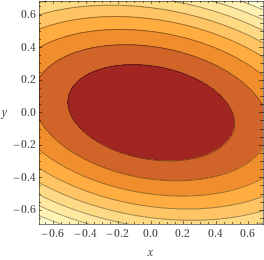
\includegraphics[width=0.5\textwidth]{./figures/Quadratic2d.png}
    \caption{$x^2 + \frac{3}{4}xy + 3y^2$}
\end{figure}

\noindent
To be rigorous, a quadratic form is a polynomial with terms that all have degree 2 (i.e. $x^2 + xy + y^2$). In general they can be written as

\begin{equation}
    \sum_{i=1}^{n} \sum_{j=1}^{n} a_{ij} x_i x_j = x^T A x
\end{equation}

\noindent
Where we assume that $A$ is symmetric. It doesn't have to be, but if it isn't, we could replace it with $(A + A^T)/2$ and get the same result.


\subsection{Norms}

A norm is a measure of how far a vector is from 0. However, there are a number of different possible norms and I keep forgetting the notation.

The $l_1$ norm, sometimes called the Manhattan norm is,

\begin{equation}
    \parallel x \parallel_1 = |x_1| + |x_2| + \cdots + |x_n|
\end{equation}

\noindent
The Euclidean norm, sometimes called the $l_2$ norm is,

\begin{equation}
    \parallel x \parallel_2 = \sqrt{x_1^2 + \cdots + x_n^2}
\end{equation}

\noindent
In general, the $p$ norm is,

\begin{equation}
    \parallel x \parallel_p = (|x_1|^p + \cdots + |x_n|^p)^{1/p}
\end{equation}


\subsection{Convex Functions}

A function, $f: R^n \rightarrow R$, is convex if its domain is a convex set and for all points $a, b \in \boldsymbol{\rm dom}\, f$ and $0 < \theta < 1$,

\begin{equation}
    f( \theta a + (1 - \theta) b ) \leq \theta f(a) + (1- \theta) f(b)
    \label{eq:JensensEquality}
\end{equation}

\noindent
which we can interpret as the value of the function between two points being on or below the straight line connecting the function's value at those two points. \autoref{eq:JensensEquality} is called ``Jensen's Equality''.
A function is {\em strictly\/} convex is we can replace $\leq$ with $<$.

\begin{figure}[h!]
    \centering
    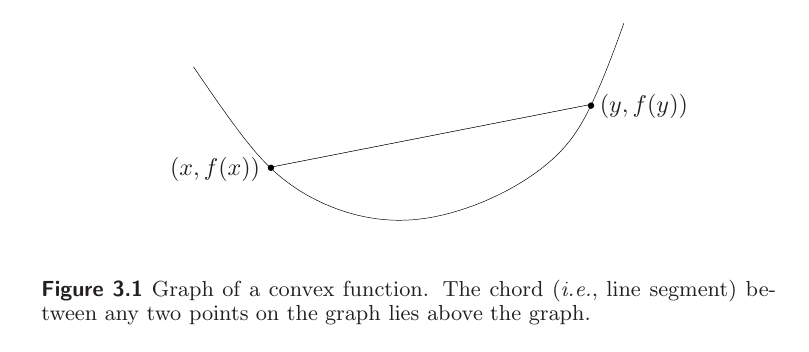
\includegraphics[width=1\textwidth]{./figures/ConvexFunction.png}
\end{figure}

Another way to think about this is to compare the behavior of the function $f$ to that of its gradient at any points.
The first order conditions say that a function is convex iff (\autoref{fig:convexFunctionGrad}),

\begin{equation}
    f(b) \geq f(a) + \nabla f(a)^T (b - a)
    \label{eq:firstOrderCondition}
\end{equation}

\begin{figure}[h!]
    \centering
    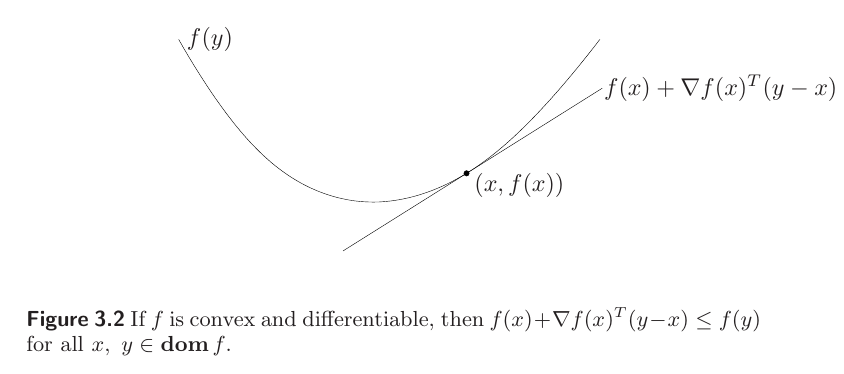
\includegraphics[width=1\textwidth]{./figures/ConvexFunctionGrad.png}
    \label{fig:convexFunctionGrad}
\end{figure}

\noindent
Thus, the first order Taylor expansion of a convex function is a global {\em underestimation\/} of the true value.

\autoref{eq:firstOrderCondition} also gives a useful result. Namely that if $\nabla f(a) = 0$, we must be at a {\em global\/} minimum.
We can't be at a maxima else for all $b$, $f(b) \leq f(a)$ and we can't be at a local minimum else for some $b$ the same would be true.
Thus to find a global minimizer of a convex function, we just need to find the location where the gradient is 0.

The second order condition is that the hessian, $H(x) = \nabla^2 f(x) \geq 0$.

\section{Optimization}

\subsection{Basic Terminology}

We express optimization problems in the standard form,

\begin{align}
    \text{minimize }   & f_0(x)                             \\
    \text{subject to } & f_i(x) \le 0, \quad i = 1 \cdots m \\
                       & h_i(x) = 0, \quad i = 1 \cdots n
\end{align}

\noindent
where
$f_0: \mathbb{R}^n \rightarrow \mathbb{R}$ is the {\em objective/cost function\/},
$x \in \mathbb{R}^n$ is the {\em optimization variable\/},
$f_i(x) \le 0$ are the {\em inequality constraints} and $f_i: \mathbb{R}^n \rightarrow \mathbb{R}$ the {\em inequality constraint functions}.
$h_i$ are as $f_i$ but replacing inequality with equality.

The set of all points for which the objective and all constraint functions are defined,

\begin{equation}
    \mathbb{D} = \bigcap_{i = 1}^{m} \dom f_i \cap \bigcap_{i = 1}^{n} \dom h_i
\end{equation}

\noindent
is the domain of the optimization problem. A point $x \in \mathbb{D}$ is {\em feasible\/}. The problem as a whole is feasible if there exists at least one feasible point, and infeasible otherwise.
The set of all feasible points it the {\em feasible/constraint set}.

\subsection{Linear Optimization}

When the objective and constraint functions are all affine, the problem is called a {\em linear problem\/}.

\begin{align}
    \text{minimize }   & c^T x + d              \\
    \text{subject to } & \boldsymbol{G} x \le h \\
                       & \boldsymbol{A} x = b
\end{align}

Note that the $d$ in the objective function does not change the problem and is often omitted. Thus we optimize the linear $c^T$ rather than the affine $c^T + d$.

\subsubsection{Linear Optimization Example}

Suppose a farmer has L hectares of land and can plant some wheat or barley on some or all of it. However, he has limited pesticide (P) and fertilizer (F). He wants to maximize the money he makes where S is the selling price. For all of these at 1 subscript indicates the value for wheat and 2 barley. How can we formulate this as a linear optimization problem?

Ignoring the matrix formulation for a moment, we know that we want to maximize,

\begin{equation}
    S_1 x_1 + S_2 x_2
\end{equation}

\noindent
subject to,
\begin{align}
    F_1 x_1 + F_2 x_2 & \leq F \\
    P_1 x_1 + P_2 x_2 & \leq P \\
    x_1 + x_2         & \leq L \\
    x_1               & \geq 0 \\
    x_2               & \geq 0
\end{align}

\noindent
This can be written in the standard form

\begin{align}
    c     & = -\begin{bmatrix}
        S_1 \\
        S_2
    \end{bmatrix} \\
    c^T x & = -(S_1 x_1 + S_2 x_2)
\end{align}

\begin{equation}
    G =
    \begin{bmatrix}
        F_1 & F_2 \\
        P_1 & P_2 \\
        1   & 1   \\
        -1  & 0   \\
        0   & -1  \\
    \end{bmatrix}
    G x =
    \begin{bmatrix}
        F_1 x_1 + F_2 x_2 \\
        P_1 x_1 + P_2 x_2 \\
        x_1  + x_2        \\
        -x_1              \\
        -x_2              \\
    \end{bmatrix}
    h = \begin{bmatrix}
        F \\
        P \\
        L \\
        0 \\
        0 \\
    \end{bmatrix}
\end{equation}

\noindent
What does this look like? The level curves of the objective function are hyperplanes (a subspace whose dimension is 1d less than its ambient space) and are orthogonal to $c$ (as the gradient of $c^T x$ is $c$).
The inequality constraints are also linear and so the feasible set is a polyhedron.

\begin{figure}[h!]
    \centering
    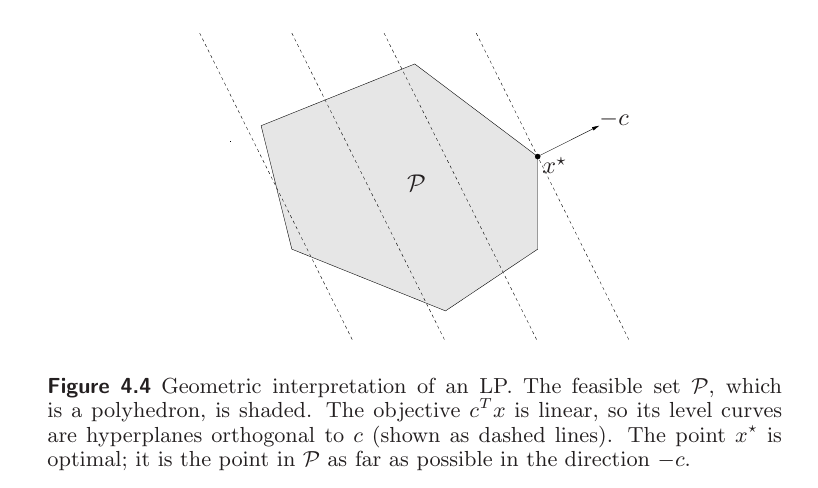
\includegraphics[width=1\textwidth]{./figures/LinearOptimizationIllustration.png}
\end{figure}

\subsection{Quadratic Optimization}

\begin{align}
    \text{minimize }   & \frac{1}{2} x^T P x + q^T x + r \\
    \text{subject to } & \boldsymbol{G} x \le h          \\
                       & \boldsymbol{A} x = b
\end{align}

\noindent
Where $P \in S^{n}_{+}$ ($n \times n$ and symmetric positive semi definite), $G \in R^{m \times n}$, and $A \in R^{k \times n}$.
Note that we could also have a {\em quadratically constrained quadratic program\/} (QCQP). In that case, as the name suggests, the constraints would be quadratic rather than linear. I'm not going to worry about that for now.

\begin{figure}[h!]
    \centering
    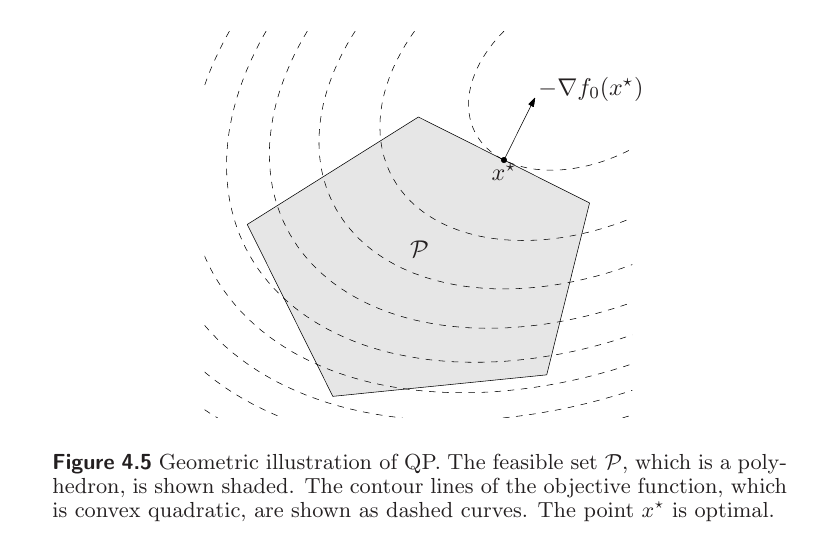
\includegraphics[width=1\textwidth]{./figures/QuadraticOptimizationIllustration.png}
\end{figure}

\subsubsection{Quadratice Optimization Example}



\section{Resources}

Convex Optimization Boyd


\bibliographystyle{plainnat}
\bibliography{/home/christopher/research/papers/all}
\end{document}
